\section{視線速度カーブからの物理量の推定}

ここまでの応用として視線速度カーブのデータ${t_i, (v_r)_i} (i=1,2,\cdots,N)$が与えられたときに、物理量$(V_\mathrm{sys}, K_\star, e, \omega, P, T_0)$を推定してみよう。まず、データ列の時間$t_i$のMean anomaly $M_i$は
\begin{align}
    M_i = (t_i - T_0) \dfrac{2 \pi}{P}
\end{align}
となる。Newton-Raphson法で$M_i$から$E_i$を求めることができる。対応するtrue anomalyは
$\cos{f_i}$, $\sin{f_i}$は
\begin{align}
    \cos{f_i} &= \dfrac{\cos{E_i}-e}{1 - e \cos{E_i}} \\
    \sin{f_i} &= \dfrac{\sin{E_i} \sqrt{1-e^2}}{1 - e \cos{E_i}} 
\end{align}
と$E$と紐付けられる。
式(\ref{eq:vrsatarefinal})より
\begin{align}
&(v_r)_{i, \mathrm{model}} = \nonumber \\
&V_\mathrm{sys} + K_\star \left[ \cos{f_i} \cos{\omega} - \sin{f_i} \sin{\omega} + e \cos{\omega} \right] 
\end{align}
となる。


確率モデルは、ここでは観測ノイズが独立ガウシアンとして
\begin{align}
    p(\dv|\thetav) &= \Ng(\muv, \sigma^2 I) \\
    \mu_i &= (v_r)_{i, \mathrm{model}} 
\end{align}
としよう。この場合、推定するパラメタは$\thetav= (V_\mathrm{sys}, K_\star, e, \omega, P, T_0, \sigma)$である。これらのパラメタの事前分布を設定することで、random MHの場合のMCMCを行うことができる。

HMC-NUTSの場合、もう少し工夫が必要である。基本的には上記のモデルをJAX等の微分可能パッケージで書けばよいが、Newton-Raphsonはwhile文と収束条件を用いて、$F(E,M,e) = E - e \sin{E} - M = 0$を解く場合、そのままでは計算グラフがつながらず微分可能でない。つまり$\partial E/\partial M$, $\partial E/\partial e$がそのままでは求まらない。
そこで陰関数定理
\begin{align}
    \dfrac{\partial E}{\partial x} = - \dfrac{ \partial F/ \partial x }{\partial F / \partial E}
\end{align}
を用いて、
\begin{align}
\dfrac{\partial E}{\partial M} &= - \dfrac{ \partial F/ \partial M }{\partial F / \partial E} = \dfrac{1}{1 - e \cos{E}} \\
\dfrac{\partial E}{\partial e} &= - \dfrac{ \partial F/ \partial e }{\partial F / \partial E} = \dfrac{\sin{E}}{1 - e \cos{E}}
\end{align}
のように手で導出した微分を自分で定義する。たとえばJAXならばcustom\_vjpを用いて、外部から微分を定義することができる。

\begin{figure}
    \centering
    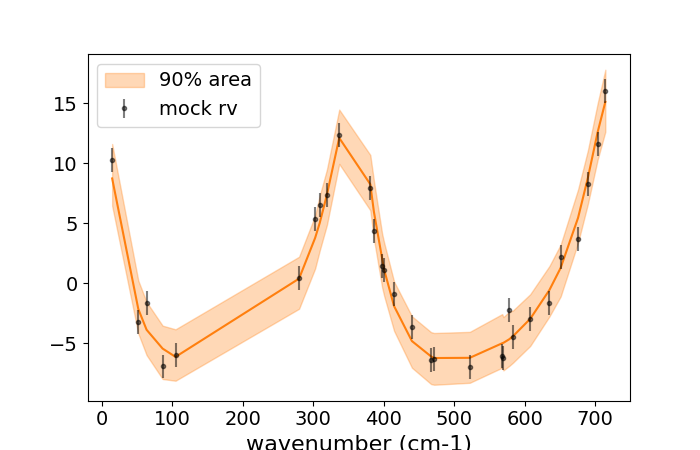
\includegraphics[width=\linewidth]{fig/rv_fit.png}
    \caption{視線速度データのフィット}
    \label{fig:rvfit}
\end{figure}